\subsection{Integrator:}

Setting the {\itshape waveform generator} in a square signal with a frequency of 1KHz and 1 $V_{pp}$ we connect the positive terminal of the {\itshape generator} to the $V_{i}$ input of the circuit of Figure 3.6.0 ( is the one on the left side of the 10 K$\Omega$ resistor ) and the negative terminal to the common ground. Then, once the respectively sources in the terminals 7 and 4 were connected, we turned-on the {\itshape generator} and the voltage sources, thus, connecting the channel 1 of the oscilloscope in the input $V_{i}$ and the channel 2 in the output $V_{o}$ we registered the waveform in Figure 3.6.1. \hfill \break

\begin{multicols}{2}
\begin{figure}[H]
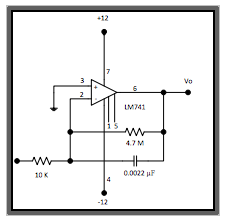
\includegraphics[width = 8cm, height = 5cm]{c6.png}
\centering \linebreak \linebreak Figure 3.6.0: Integrator circuit.
\end{figure}

\begin{figure}[H]
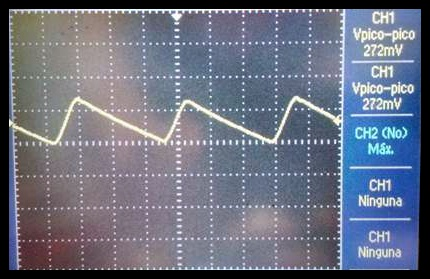
\includegraphics[width = 8cm, height = 5cm]{o6.jpg}
\centering \linebreak \linebreak Figure 3.6.1: Input and output waveform.
\end{figure}
\end{multicols} \hfill

{\bfseries\itshape\color{carmine}{Observation:}} {\itshape\color{carmine}{The input waveform is a square wave, as an effect of the integration the output waveform is a triangle wave.}}